%\documentclass[referee,pdflatex,sn-basic]{sn-jnl}
%\documentclass[sn-basic]{sn-jnl}
%\documentclass[lineno,pdflatex,sn-basic]{sn-jnl}
%\documentclass[pdflatex,sn-nature]{sn-jnl}
%\documentclass[pdflatex,sn-basic]{sn-jnl}
%\documentclass[pdflatex,sn-mathphys-num]{sn-jnl}
%\documentclass[sn-mathphys-num,iicol]{sn-jnl}
%\documentclass[pdflatex,sn-mathphys-ay]{sn-jnl}
%\documentclass[pdflatex,sn-vancouver-num]{sn-jnl}
%\documentclass[sn-mathphys-num,iicol]{sn-jnl}
\documentclass[pdflatex,sn-mathphys-num]{sn-jnl}
%\documentclass[pdflatex,sn-mathphys-num,iicol]{sn-jnl}

% Standard packages required.
\usepackage{graphicx}
\usepackage{booktabs}
\usepackage{array}
\usepackage{multirow}
\usepackage{tabularx}
\usepackage{amsmath,amssymb,amsfonts}
\usepackage{xurl}
\usepackage{afterpage}
\usepackage{float}
% Clean by default; define \ShowRevisionHighlights for yellow markup.
% Keep identical box geometry in both modes to preserve approved page references.
\usepackage{soul}
\usepackage{capt-of}
\usepackage{tcolorbox}
\tcbuselibrary{breakable,skins}
\usepackage{colortbl}
\newif\ifrevisionhighlight
\revisionhighlighttrue
\ifdefined\ShowRevisionHighlights
\definecolor{revisionyellow}{RGB}{255,245,153}
\else
\definecolor{revisionyellow}{RGB}{255,255,255}
\fi
\sethlcolor{revisionyellow}
\DeclareRobustCommand{\rev}[1]{\ifrevisionhighlight\ifmmode\mbox{\hl{#1}}\else\hl{#1}\fi\else#1\fi}
\newenvironment{revisionblock}{\ifrevisionhighlight\begin{tcolorbox}[enhanced,breakable,colback=revisionyellow,colframe=revisionyellow,boxrule=0pt,arc=0pt,outer arc=0pt,left=0pt,right=0pt,top=2pt,bottom=2pt,boxsep=0pt,before skip=5pt,after skip=5pt]\fi}{\ifrevisionhighlight\end{tcolorbox}\fi}
\newcommand{\revisionrow}{\ifrevisionhighlight\rowcolor{revisionyellow}\fi}
\AtBeginDocument{\pdfstringdefDisableCommands{\def\rev#1{#1}}}
\newcommand{\revisioncell}[1]{\ifrevisionhighlight\cellcolor{revisionyellow}\fi#1}


%\usepackage[margin=3cm]{geometry}

\geometry{margin=2.2cm}
\usepackage{setspace}
\setstretch{1.2}

% Manuscript macros.
\newcommand{\figref}[1]{Fig.~\ref{#1}}
\newcommand{\tabref}[1]{Table~\ref{#1}}
\newcommand{\eqnref}[1]{Eq.~\eqref{#1}}
\newcommand{\pmid}[1]{\href{https://pubmed.ncbi.nlm.nih.gov/#1/}{PMID:#1}}
\newcommand{\doi}[1]{\href{https://doi.org/#1}{\mbox{doi:\nolinkurl{#1}}}}
\newcommand{\softfuse}{SoftFuse-KGC}
\newcommand{\drkgc}{DrKGC}
\newcommand{\kgc}{knowledge graph completion}
\newcommand{\bkg}{biomedical knowledge graph}
\newcommand{\topk}{top 20}
\newcommand{\mrr}{MRR@20}

\raggedbottom

\hypersetup{
  pdftitle={SoftFuse-KGC: Soft Support and Confidence-Aware Fuzzy Retrieval for Biomedical Knowledge Graph Completion},
  pdfauthor={Dang Hoang Duong, Le Van Thanh, Hai Van Pham},
  pdfsubject={Original research article},
  pdfkeywords={Biomedical knowledge graph; Knowledge graph completion; Drug repurposing; Soft evidence modeling; Fuzzy retrieval},
  bookmarksdepth=2
}

\begin{document}

\title[SoftFuse-KGC for biomedical knowledge graph completion]{SoftFuse-KGC: Soft Support and Confidence-Aware Fuzzy Retrieval for Biomedical Knowledge Graph Completion}

\author[1,2]{Le Van Thanh}\email{thanhlv@vinhuni.edu.vn}
\author[3]{Dang Hoang Duong}\email{duong.dh235922@sis.hust.edu.vn}
\author*[3]{Hai Van Pham}\email{haipv@soict.hust.edu.vn}


\affil[1]{\orgdiv{School of Engineering and Technology}, \orgname{Vinh University}, \state{Nghean}, \country{Vietnam}}
\affil[2]{\orgname{Graduate University of Science and Technology, Vietnam Academy of Science and Technology}, \city{Hanoi}, \country{Vietnam}}
\affil[3]{\orgdiv{School of Information and Communications Technology}, \orgname{Hanoi University of Science and Technology}, \city{Hanoi}, \country{Vietnam}}

\abstract{Biomedical knowledge graph completion can support drug repurposing, but graph-augmented large language model (LLM) pipelines are sensitive to poorly ordered candidates and noisy query-specific evidence. In this paper, we \rev{present} \softfuse, an evidence-calibration framework for drug-focused link prediction with graph-augmented LLMs. \rev{The soft-support module} reranks top-20 candidates using graded evidence contact, mechanism-oriented support, and penalties for direct shortcuts and contradictory signals. Its confidence-aware fuzzy retriever selects a compact evidence graph using rank confidence, query and candidate incidence, penalty signals, and local density while preserving candidate order. We evaluate the framework on PrimeKG, PharmKG, Hetionet, the Drug Repurposing Knowledge Graph (DRKG), and repoDB. On PrimeKG, \softfuse{} raises candidate mean reciprocal rank at 20 (MRR@20) from 0.0646 to 0.1253 and end-to-end MRR@20 from \rev{0.0477} to 0.0747 while reducing the average graph from 59.93 to 32.34 triples. On PharmKG, it raises end-to-end MRR@20 from 0.0156 to 0.0210 and reduces the graph from 100 to 55 triples. \rev{On Hetionet, DRKG, and repoDB, fuzzy retrieval reduces average graph size by 45\% while retaining or improving end-to-end MRR@20 relative to the uncompressed input. Further analyses show that learned and transferred coefficients can improve candidate ranking, although gains vary across datasets. Comparisons at matched graph budgets also reveal a trade-off between candidate coverage and path retention.} These results show that candidate calibration and evidence compression offer complementary benefits whose effectiveness depends on graph topology and query-specific support. \rev{Two detailed PrimeKG case studies illustrate how the modules change candidate ranks and retain relevant graph evidence. A web interface supports inspection of these changes through candidate support scores, ranking comparisons, and retrieved subgraphs.}}

\keywords{Biomedical knowledge graph \textperiodcentered\ Knowledge graph completion \textperiodcentered\ Drug repurposing \textperiodcentered\ Soft evidence modeling \textperiodcentered\ Fuzzy retrieval}

\maketitle

% =========================================================
% 1. Introduction
% =========================================================

\section{Introduction}
\label{sec:introduction}

Knowledge graphs (KGs) represent entities and their typed relations in a form that supports integrating, analyzing, and reasoning over heterogeneous knowledge \citep{nickel2015review,ji2021survey,hogan2021knowledge}. This representation is particularly useful in biomedicine, where relevant evidence is distributed across drugs, diseases, genes, proteins, pathways, adverse events, phenotypes, and molecular mechanisms. Biomedical knowledge graphs (BKGs) and related resources, including Hetionet~\citep{himmelstein2017systematic}, PrimeKG~\citep{chandak2023building}, PharmKG~\citep{zheng2021pharmkg}, DRKG~\citep{drkg2020}, repoDB~\citep{brown2017standard}, and others organize this evidence into computable graph structures for translational discovery, drug repurposing, safety modeling, and therapeutic hypothesis generation. These resources integrate biomedical terminologies and molecular databases such as UMLS~\citep{bodenreider2004unified}, DisGeNET~\citep{pinero2020disgenet}, UniProt~\citep{uniprot2018uniprot}, OMIM~\citep{amberger2019omim}, DrugBank~\citep{wishart2018drugbank}, STITCH~\citep{kuhn2014stitch}, and STRING~\citep{szklarczyk2021string}. Despite their broad coverage, curated BKGs remain incomplete. Biomedical facts may be missing from databases, dispersed across publications, represented with inconsistent identifiers, or not yet known.

Knowledge graph completion (KGC), often formulated as link prediction, addresses this incompleteness by ranking plausible missing triples from the observed graph \citep{nickel2015review,ji2021survey,wang2017knowledge}. Many established KGC methods rely primarily on graph structure. Translation and semantic matching models such as TransE~\citep{bordes2013translating}, DistMult~\citep{yang2014embedding}, ComplEx~\citep{trouillon2016complex}, and RotatE~\citep{sunrotate} learn representations of entities and relations and use them to score candidate triples efficiently. Graph neural networks such as R-GCN~\citep{schlichtkrull2018modeling} and CompGCN~\citep{vashishthcomposition}, together with relation-aware graph attention models~\citep{sheikh2021knowledge}, extend this approach by aggregating information from multirelational neighborhoods, allowing local graph context and multi-hop biomedical evidence to influence prediction. Rule-based and path-based methods provide more interpretable predictions through relational patterns and mechanistic paths. However, these methods can become brittle when biomedical evidence is sparse or when the graph does not contain a useful path \citep{yang2017differentiable,meilicke2019anytime,cheng2023neural}.

Textual information provides another source of evidence for biomedical KGC. Entity names, relation labels, and biomedical descriptions contain semantic information that structure-only models may not capture. Language-model-based KGC and text-enhanced ranking methods therefore use relation descriptions, entity names, instruction prompts, retrieval, or candidate-constrained generation to connect graph prediction with biomedical language \citep{devlin2019bert,gu2021domain,luo2022biogpt,wang2022simkgc,wei2026kicgptv2,zhang2024making,liu2024finetuning,wang2024kc}. More recent graph-augmented LLM systems combine candidate retrieval, graph evidence retrieval, graph adapters, and parameter-efficient fine-tuning so that generation can be conditioned more directly on retrieved graph evidence. \drkgc{}~\citep{xiao2025drkgc} represents this direction by integrating question templates, lightweight candidate retrieval, rule-guided subgraph retrieval, graph-adapter embeddings, and LoRA~\citep{hulora} fine-tuning. For biomedical applications, this design provides a language-based prediction interface while retaining structured evidence from the graph.

The connection between retrieval and generation nevertheless creates two important bottlenecks. First, a candidate-constrained LLM can select only from the entities provided by the candidate retriever. If the gold drug is absent from the top-\(K\) candidate list, the generation stage cannot recover it. Even when the gold drug is present, a position near the end of the list may limit its influence on generation and make the prediction less useful for manual review. Second, the graph adapter can use only the evidence contained in the retrieved subgraph. A large or noisy graph may be dominated by direct shortcuts, frequently connected entities, or relations that are structurally close to the query but offer limited clinical or mechanistic information. These limitations are especially relevant to therapeutic head prediction, in which the system ranks drugs or compounds for an incomplete triple of the form $(?,r,\mathrm{disease})$. Evidence for such a query may be indirect and may involve drug targets, disease-associated genes, protein interactions, pathways, previous indications, failed indications, or literature-derived associations.

These retrieval constraints motivate a graded treatment of biomedical evidence. A drug--target edge, disease--gene association, protein interaction, therapeutic association, approved indication, and contraindication-like signal provide different types and strengths of evidence. At the same time, the absence of a path in an incomplete BKG should not automatically be interpreted as negative evidence. Although hard filters are easy to inspect, they may remove recoverable candidates simply because the graph lacks a particular supporting edge. Fuzzy set theory introduced graded membership as an alternative to binary inclusion \citep{zadeh1965fuzzy}, and fuzzy logic subsequently provided formal tools for reasoning with partial truth and uncertainty \citep{prade1980fuzzy,hajek2001metamathematics,straccia2006fuzzy,lukasiewicz2008managing}. Applied to biomedical graph-LLM completion, this perspective suggests that candidate support and graph evidence should be calibrated according to their degree of support, their susceptibility to shortcut behavior, and the confidence associated with the retrieved context.

We address this retrieval--generation interface with \softfuse, an evidence-calibration framework for \drkgc{}-style biomedical graph-augmented LLM completion. \softfuse{} contains two complementary modules. The soft support module reranks retrieved drug candidates using graded evidence contact, mechanism-oriented support, penalties for direct shortcuts, and contradiction cues. The confidence-aware fuzzy retrieval module selects a compact evidence subgraph using candidate rank bands, candidate and query incidence, relation-family priorities, local density, and penalty signals, while preserving the selected candidate order. \softfuse{} is not intended to replace the upstream structural candidate generator. Instead, it evaluates three distinct aspects that are often conflated in graph-LLM pipelines: gold-candidate recoverability, the ordering of recoverable candidates, and the compactness and auditability of the evidence supplied to the graph adapter.

\rev{The contribution is the integration and evaluation of explicit biomedical evidence cues at the candidate--graph interface, building on established reranking and subgraph-selection principles.} The main contributions of this paper are as follows:
\begin{itemize}
\item \rev{We formulate an inspectable soft-support reranker for a fixed top-20 biomedical candidate set, combining evidence contact with shortcut and contradiction penalties.}
\item \rev{We develop a confidence-aware fuzzy retrieval module that combines rank-aware edge scoring with coverage-first selection to construct compact evidence graphs while preserving candidate order.}
\item \rev{We evaluate the framework on five biomedical datasets, examining candidate ranking, end-to-end performance, and evidence-graph size across different graph structures and therapeutic relations.}
\item \rev{We provide PrimeKG case studies spanning three diagnostic categories, including two detailed examples of candidate reranking and evidence selection. We also provide a web application for reproducible inspection of candidate support, rank changes, and selected evidence.}
\end{itemize}

The remainder of this paper is organized as follows. Section~\ref{sec:related} reviews structure-based biomedical KGC, graph-augmented LLMs, and soft evidence modeling. Section~\ref{sec:methods} presents the \softfuse{} framework, including its graph-LLM backbone, soft support module, fuzzy retrieval module, and graph-adapter-enhanced generation. Section~\ref{sec:results} describes the study datasets and evaluation metrics before reporting the candidate-stage, end-to-end, case-study, and web-server results. Section~\ref{sec:discussion} discusses the findings and limitations. Section~\ref{sec:conclusion} concludes the paper and outlines future research directions.


% =========================================================
% 2. Related Work
% =========================================================

\section{Related Work}
\label{sec:related}

\subsection{Structure-based biomedical KGC}

Translation and semantic matching models such as TransE~\citep{bordes2013translating}, DistMult~\citep{yang2014embedding}, ComplEx~\citep{trouillon2016complex}, and RotatE~\citep{sunrotate} represent entities and relations in continuous embedding spaces and score candidate triples from these representations. Their efficient scoring functions make them useful as large-scale candidate generators, although their predictions are driven mainly by structural regularities in the observed graph. Graph neural networks such as R-GCN~\citep{schlichtkrull2018modeling} and CompGCN~\citep{vashishthcomposition}, together with relation-aware graph attention variants~\citep{sheikh2021knowledge}, incorporate information from multirelational neighborhoods into entity representations. These models represent local relational context more explicitly than conventional embedding models. Rule-based and path-based approaches instead identify interpretable relational patterns or paths that connect candidate entities to a query. Their dependence on observable paths, however, can make them sensitive to missing evidence \citep{yang2017differentiable,meilicke2019anytime,cheng2023neural}. Biomedical link prediction and drug repurposing studies further demonstrate that graph proximity must be interpreted carefully because structural closeness alone does not establish therapeutic appropriateness \citep{himmelstein2017systematic,sadegh2020exploring,ashburn2004drug,pushpakom2019drug}.


\begin{revisionblock}
Recent graph-based drug-repositioning methods combine complementary biological networks to capture associations at multiple scales. For example, Zhu et al.~\citep{zhu2026spatialspectral} combine wave-based propagation and spectral transforms to model similarity and drug--protein--disease networks. Their framework uses contrastive learning to align local and global representations. Similarly, FD-MSGL~\citep{zhu2026fdmsgl} uses frequency-domain graph learning to combine molecular similarity, drug--target interactions, and regulatory pathways. By integrating these complementary sources, both approaches represent indirect associations that may be missed when a single network is used.
\end{revisionblock}

\subsection{Text and graph-augmented LLMs}

Text-enhanced and LLM-based KGC methods use relation descriptions, entity names, instruction tuning, retrieval, or candidate-constrained generation to complement structural graph information \citep{devlin2019bert,gu2021domain,luo2022biogpt,wang2022simkgc,wei2026kicgptv2,zhang2024making,liu2024finetuning,wang2024kc}. This approach is relevant to BKGs because biomedical entity names and relation labels contain domain-specific semantic information. Text-only prompting, however, may omit important graph structure, whereas unconstrained generation can produce entities that do not belong to the graph or the intended candidate set.

\drkgc{}~\citep{xiao2025drkgc} is particularly relevant to the present study because it combines question templates, lightweight candidate retrieval, rule-guided dynamic subgraph retrieval, graph-adapter embeddings, and LoRA~\citep{hulora} fine-tuning. Related biomedical graph-LLM research also shows the value of combining textual representations with domain-specific graph evidence \citep{xiao2024fuselinker}. Nevertheless, a \drkgc{}-style system remains dependent on two retrieved inputs: the ordered candidate list and the query-specific evidence graph supplied to the graph adapter. Errors in either input can propagate to candidate-constrained generation.

More broadly, retrieval-augmented generation treats external evidence as a non-parametric memory for knowledge-intensive tasks, allowing a generator to use retrieved context in addition to information stored in its parameters \citep{lewis2020retrieval}. Surveys of KG--LLM integration similarly distinguish KG-enhanced LLMs, LLM-augmented KGs, and systems that combine the two components more closely \citep{pan2024unifying}. In biomedical KGC, these research directions highlight a practical problem at the retrieval--generation interface: prioritizing retrieved candidates and allocating the limited evidence budget to the most relevant local triples.

\subsection{\rev{Evidence reranking and compact subgraph retrieval}}
\begin{revisionblock}
Evidence reranking helps retrieval-augmented models prioritize the context supplied to a generator. RankRAG~\citep{yu2024rankrag} instruction-tunes a single LLM for both retrieved-context ranking and answer generation, integrating evidence prioritization into the generation pipeline. For graph-structured evidence, G-Retriever~\citep{he2024gretriever} selects relevant context through prize-collecting Steiner-tree optimization and conditions an LLM with graph representations. GRAG~\citep{hu2025grag} also retrieves textual subgraphs, combining graph and text views for generation. At the triple level, SubgraphRAG~\citep{li2025subgraphrag} learns parallel triple scores with a lightweight multilayer perceptron and directional structural features, allowing the retrieved graph size to vary with the evidence budget. Together, these methods show how context ranking and subgraph selection can organize relevant evidence within a limited retrieval budget.
\end{revisionblock}

\subsection{Soft evidence for graph-LLM completion}

Soft evidence modeling is appropriate for this setting because biomedical graph relations are heterogeneous. A drug--target edge, disease--gene association, protein interaction, literature-derived drug--disease association, and approved indication do not provide equivalent therapeutic evidence. Hard filtering remains interpretable, but it can be unreliable in an incomplete BKG: The absence of an observed supporting relation does not necessarily indicate the absence of biomedical support. Fuzzy set theory represents membership as a degree rather than a binary decision \citep{zadeh1965fuzzy}, while fuzzy logic provides foundations for reasoning with partial truth and uncertainty \citep{prade1980fuzzy,hajek2001metamathematics,straccia2006fuzzy,lukasiewicz2008managing}. Fuzzy knowledge graphs have also been combined with complex fuzzy inference systems to support approximate reasoning when the available knowledge or rule base is limited \citep{lan2020complexfkg}. In clinical decision support, picture fuzzy sets and knowledge-based reasoning have been used to represent imprecise diagnostic information \citep{pham2022picturefuzzyclinical,khan2026novel}.

% =========================================================
% 3. Methods
% =========================================================

\section{Methods}
\label{sec:methods}

\subsection{\drkgc{}-style graph-LLM backbone}

The backbone retains the central components of \drkgc{}~\citep{xiao2025drkgc}: candidate retrieval, source-subgraph retrieval, graph-adapter embedding enhancement, and candidate-constrained LLM prompting. Across all datasets, we use a lightweight R-GCN~\citep{schlichtkrull2018modeling} ranker as the graph-compatible source. This choice is motivated by interface compatibility rather than by an assumption that R-GCN is the strongest standalone link predictor. R-GCN provides relation-aware entity embeddings and local neighborhoods in the format expected by the \drkgc{}-style subgraph encoder. Using the same source also keeps the graph-adapter interface fixed and makes the calibration modules comparable across datasets.

The calibration modules themselves are not tied to R-GCN. Any structural or hybrid retriever can serve as the source if it provides a fixed candidate list, compatible entity identifiers or embeddings, and a query-specific subgraph. Integrating stronger compatible sources, such as ComplEx~\citep{trouillon2016complex}, DistMult~\citep{yang2014embedding}, relation-aware attention retrievers~\citep{sheikh2021knowledge}, or hybrid retrievers, remains future work. The initial candidate list is defined as follows:
\begin{equation}
C^{(0)}_q=(c_1,c_2,\ldots,c_K), \quad K=20,
\label{eq:candidate_list}
\end{equation}
where the backbone structural score determines the order. Candidate names are inserted explicitly into the prompt, which instructs the LLM to return one entity from this set. The source subgraph is intentionally larger than the final fuzzy graph. This design preserves the original \drkgc{} graph-adapter interface while retaining enough local evidence for \softfuse{} to determine which candidate and edge signals should be retained or downweighted.

\subsection{Overview of the \softfuse{} framework}

\softfuse{} operates as an evidence-calibration layer between candidate retrieval and graph-adapter-enhanced generation. \figref{fig:framework} shows the four implementation stages. \textbf{A. Biomedical backbone preparation} constructs the task-specific BKG, trains or loads the graph-compatible drug ranker, exports global entity embeddings, and prepares path rules and question templates. \textbf{B. Candidate and evidence retrieval} receives a therapeutic query of the form $(?,r_q,\mathrm{disease})$, retrieves the top-20 drug candidates, and packages a source subgraph containing direct candidate--query edges, candidate neighborhoods, and rule-compatible local paths. \textbf{C. \softfuse{} evidence calibration} applies the two proposed modules: C1 soft support reranks candidates from graded support and penalty cues, whereas C2 confidence-aware fuzzy retrieval selects a smaller evidence graph using rank-band confidence and edge-level evidence quality. \textbf{D. Graph-enhanced candidate-constrained generation} passes the calibrated candidates and selected graph to the graph adapter and LoRA-tuned LLM, which must return one supplied candidate.

The distinction between C1 and C2 is central to the study design. We attribute changes in candidate order to soft support and changes in graph size or evidence content to fuzzy retrieval. 

\begin{figure*}[!tbp]
\centering
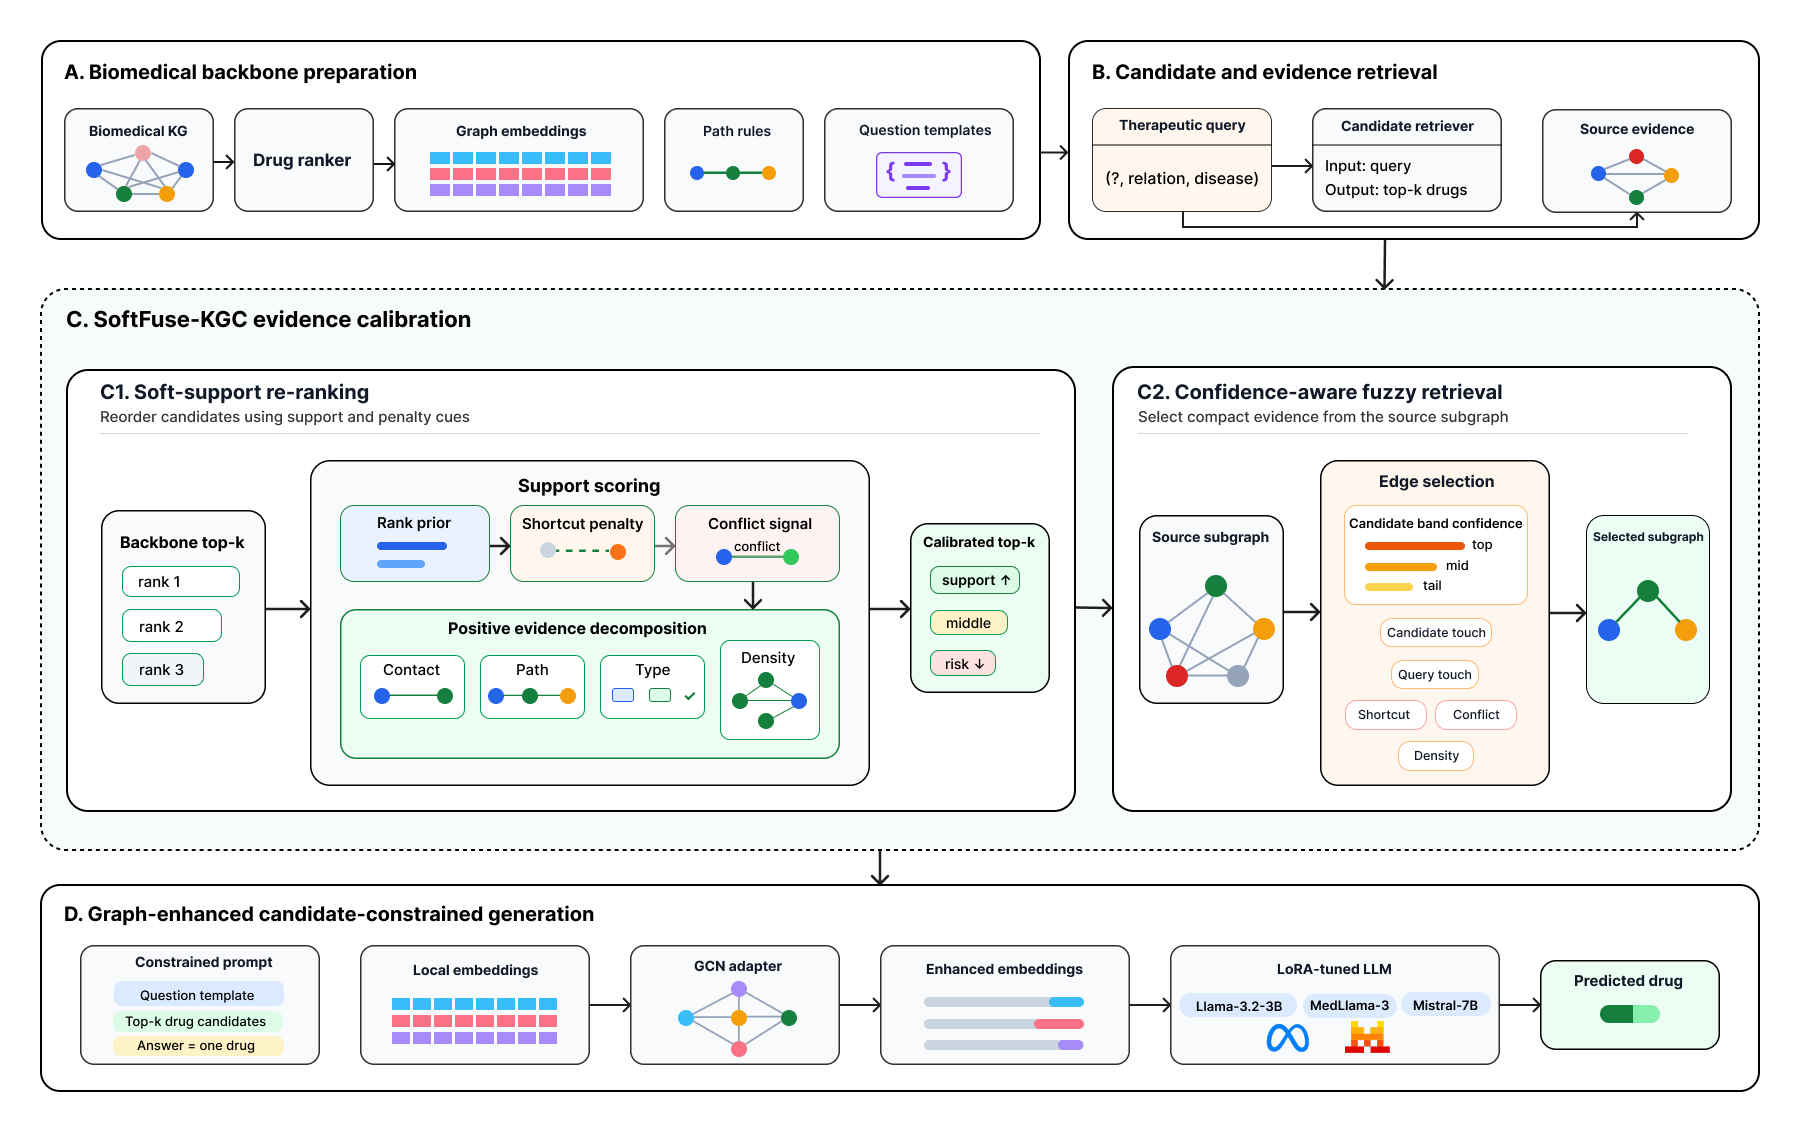
\includegraphics[width=\textwidth]{Fig1.png}
\caption{\textbf{\softfuse{} framework for evidence-calibrated biomedical graph-augmented LLM completion.} \textbf{A. Biomedical backbone preparation} builds the BKG, graph-compatible drug ranker, graph embeddings, path rules, and question templates. \textbf{B. Candidate and evidence retrieval} converts a therapeutic query into a top-20 candidate list and source evidence subgraph. \textbf{C. \softfuse{} evidence calibration} includes C1 soft support reranking, which combines a rank prior, decomposed positive support, shortcut penalties, and contradiction signals, and C2 confidence-aware fuzzy retrieval, which selects compact evidence using candidate bands, candidate and query incidence, shortcut, conflict, and density cues. \textbf{D. Graph-enhanced candidate-constrained generation} passes the calibrated candidates and selected graph through the graph adapter and LoRA-tuned LLM to predict one drug}
\label{fig:framework}
\end{figure*}

\subsection{Soft support candidate reranking}

The soft support module reranks the backbone candidates using evidence extracted from the initial source subgraph $S^{(0)}_q$. This is the graph package constructed by the \drkgc{}-style retriever before fuzzy compression. It contains candidate--query paths, candidate-neighborhood edges, and relation-specific evidence that may provide support, indicate risk, or create an ambiguous connection between a candidate and the query. Soft support converts these heterogeneous signals into a calibrated candidate score rather than making a binary keep-or-discard decision.

We formulate soft support as a unified candidate score. It combines positive evidence $E_i(q)$, direct-shortcut or popularity evidence $D_i(q)$, contradiction-like evidence $X_i(q)$, and, where selected, a backbone rank prior. Dataset-specific instantiations set the coefficients of unavailable or inactive terms to zero.

For query $q$ and candidate $c_i$, the positive support family is computed as follows:
\begin{equation}
\begin{aligned}
E_i(q)=&
\omega_{\mathrm{touch}}T_i(q)+\omega_{\mathrm{path}}P_i(q)\\
&+\omega_{\mathrm{schema}}A_i(q)+\omega_{\mathrm{density}}\Delta_i(q),
\end{aligned}
\label{eq:evidence_support}
\end{equation}
where $T_i(q)$ denotes candidate evidence contact, $P_i(q)$ denotes mechanism-oriented path support, $A_i(q)$ denotes type or schema compatibility, and $\Delta_i(q)$ denotes local evidence density. A contact-based instantiation uses $T_i(q)=\mathbb{I}[\deg_{S^{(0)}_q}(c_i)>0]$, where $\deg_{S^{(0)}_q}(c_i)$ counts source-subgraph triples incident to the candidate. In this setting, $P_i(q)$ summarizes shared-gene overlap, gene--gene bridge evidence, and contacts with candidate- and query-side mechanism neighborhoods:
\begin{equation}
\begin{aligned}
P_i(q)=&
\nu_sM^s_i(q)+\nu_bM^b_i(q)\\
&+\nu_cT^c_i(q)+\nu_qT^q_i(q),\\
M^s_i(q)=&
\min\left(1,\frac{|G(c_i)\cap G(q)|}{\eta_s}\right),\\
M^b_i(q)=&
\min\left(1,\frac{B_i(q)}{\eta_b}\right),
\end{aligned}
\label{eq:path_support}
\end{equation}
where $G(c_i)$ is the set of target or associated genes for the compound, $G(q)$ is the disease-gene set, and $B_i(q)$ counts gene--gene bridge edges between these sets. The terms $T^c_i(q)$ and $T^q_i(q)$ indicate whether the source subgraph contains candidate-side and query-side mechanism neighborhoods, respectively. Schema support is defined as follows:
\begin{equation}
A_i(q)=
\mathbb{I}[\tau(c_i)\in\mathcal{T}_{\mathrm{drug}}]\,
\mathbb{I}[\tau(t_q)\in\mathcal{T}_{\mathrm{disease}}],
\label{eq:schema_support}
\end{equation}
when entity-type annotations are available. The density term is a bounded local count, for example,
\begin{equation}
\Delta_i(q)=
\min\left(1,\frac{\log(1+\deg_{S^{(0)}_q}(c_i)+\deg_{S^{(0)}_q}(t_q))}{\eta_\Delta}\right).
\label{eq:density_support}
\end{equation}
Together, these components make $E_i(q)$ a positive evidence score rather than a detector of a single direct link.

The two penalty terms represent different failure modes. The first, $D_i(q)$, captures a direct shortcut or candidate-level popularity:
\begin{equation}
D_i(q)=
\max\left(
\mathbb{I}[c_i \leftrightarrow t_q \text{ in } S^{(0)}_q],
\min\left(1,\frac{\deg_{\mathrm{direct}}(c_i)}{\eta_D}\right)
\right),
\label{eq:shortcut_penalty}
\end{equation}
The first component detects a direct candidate--query edge in the source graph. The second penalizes candidates that act as generic hubs across direct disease relations. The contradiction term $X_i(q)$ marks contraindication, conflict, failed, or suspended-indication evidence:
\begin{equation}
X_i(q)=\mathbb{I}[c_i \leftrightarrow t_q \text{ through contradiction-like evidence}].
\label{eq:conflict_penalty}
\end{equation}

We first compute an evidence-only score and then, when selected, combine its within-query normalized value with the backbone rank prior:
\begin{equation}
\begin{aligned}
\widetilde{S}_{\theta_d}(c_i,q)=&
\alpha_{E,d}E_i(q)
-\alpha_{D,d}D_i(q)
-\alpha_{X,d}X_i(q),\\
S_{\theta_d}(c_i,q)=&
\mu_d R_i(q)+(1-\mu_d)N_q\!\left(\widetilde{S}_{\theta_d}(c_i,q)\right).
\end{aligned}
\label{eq:soft_general}
\end{equation}
Here, $R_i(q)=(K-r_i^{(0)}+1)/K$ is the normalized backbone rank prior. The function $N_q(\cdot)$ is the within-query normalization when a rank-prior mixture is selected and the identity map otherwise. The index $d$ denotes the dataset, and $\theta_d$ collects its calibration parameters.

Candidates are sorted by decreasing soft support score, with the original backbone rank used as a stable tiebreaker:
\begin{equation}
c_i \prec c_j
\Longleftrightarrow
S_i>S_j
\quad \mathrm{or}\quad
(S_i=S_j \ \mathrm{and}\ r^{(0)}_i<r^{(0)}_j),
\label{eq:tie_break}
\end{equation}
where $S_i=S_{\theta_d}(c_i,q)$ and $r^{(0)}_i=\mathrm{rank}_0(c_i)$. We denote the resulting candidate list by $C^{\mathrm{soft}}_q$.

Online Resource 1 provides the feature-selection procedure, weight-assignment method, saturation constants, normalization choices, and validation-frozen coefficients for equations \eqref{eq:evidence_support}--\eqref{eq:soft_general}. Supplementary Section S1 describes the soft-support feature audit and coefficient assignment, Table S1 reports the dataset-specific instantiations, and Supplementary Section S6 summarizes the PrimeKG formula variants used as representative ablations.

\figref{fig:soft} presents a validation-level view of this behavior on PrimeKG. Panel A compares candidate-ranking metrics for the raw backbone, ontology filtering, a contrastive support variant, and the selected soft support setting. Ontology filtering serves as the hard-filter control: candidates are retained only when they satisfy binary type, schema, or ontology-support conditions, while candidates without such support are discarded or demoted. This control is diagnostically useful but can be brittle in an incomplete BKG because missing ontology evidence is not equivalent to negative biomedical evidence. By contrast, the selected soft support setting retains all top-20 candidates and changes only their order. Panel B shows that this setting improves validation ranking while lowering the top-five direct-link rate. The comparison therefore supports the interpretation that the gain reflects graded evidence calibration rather than the promotion of shortcut-connected candidates.

\begin{figure*}[!t]
\centering
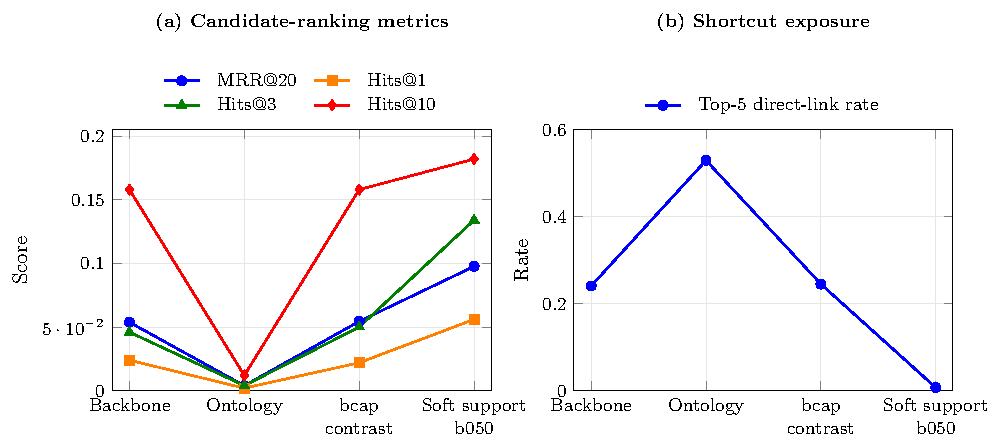
\includegraphics[width=\textwidth]{Fig2_revised.pdf}
\caption{\rev{Soft-support calibration and shortcut exposure on the PrimeKG validation set. Panel (a) compares candidate-ranking metrics for the raw backbone, hard ontology filtering, capped-evidence contrast, and the selected soft-support setting (b050); absent gold candidates receive zero reciprocal rank. Panel (b) shows the top-five direct-link rate for the same settings. Soft support raises validation MRR@20 from 0.0538 to 0.0976 while reducing this rate from 0.2408 to 0.0072.}}
\label{fig:soft}
\end{figure*}

\subsection{Confidence-aware fuzzy retrieval}

The fuzzy retrieval module changes the evidence graph supplied to the graph adapter while preserving a validation-selected candidate order. Let $C^{\mathrm{in}}_q$ denote this fixed input list. In the main pipeline, it is usually the soft-support list; the protocol can instead use a backbone-compatible list when validation analysis indicates that soft support should remain diagnostic rather than define the main row. Let $S^{(0)}_q$ denote the source evidence subgraph for query $q$, and let $e=(u,r,v)$ be an evidence triple. Fuzzy retrieval assigns a confidence-aware score to every edge and selects a compact subgraph $S^{\mathrm{fuzzy}}_q$ under a dataset-specific graph budget.

A key component is candidate rank-band confidence. Under the fixed top-20 protocol, the selected list is partitioned into ordered bands for the highest-ranked, middle, and recoverable tail candidates. When an edge touches one or more candidates, its band score is the largest weight assigned to any touched candidate:
\begin{equation}
B(e,q)=\max_{c_i\in C^{\mathrm{in}}_q: e\sim c_i} w_b(r_i),
\label{eq:band}
\end{equation}
and we set $B(e,q)=0$ when $e$ touches no candidate. Here, $e\sim c_i$ means that edge $e$ is incident to candidate $c_i$ or is annotated as part of a candidate-anchored evidence path; $r_i$ is the selected rank of $c_i$.

The confidence-aware edge score combines rank-band confidence $B(e,q)$, candidate incidence $T^c_e(q)$, query incidence $T^q_e(q)$, a top-candidate bonus $H_e(q)$, a direct-shortcut penalty $D_e(q)$, a contradiction or failed-evidence penalty $X_e(q)$, local density $\rho_e(q)$, and relation-family priority $F_r(e)$. Dataset-specific instantiations give zero coefficients to unavailable or inactive terms.

The full edge score is computed as follows:
\begin{equation}
\begin{aligned}
S_{\mathrm{edge}}(e,q)=&
\lambda_fF_r(e)+\lambda_bB(e,q)+\lambda_cT^c_e(q)\\
&+\lambda_qT^q_e(q)+\lambda_{\mathrm{top}}H_e(q)-\lambda_dD_e(q)\\
&-\lambda_xX_e(q)+\lambda_{\rho}\rho_e(q),
\end{aligned}
\label{eq:edge_score}
\end{equation}
where
\begin{equation}
\begin{aligned}
T^c_e(q)&=
\mathbb{I}[u\in C^{\mathrm{in}}_q \ \mathrm{or}\ v\in C^{\mathrm{in}}_q],\\
T^q_e(q)&=
\mathbb{I}[u=t_q \ \mathrm{or}\ v=t_q],\\
H_e(q)&=
\mathbb{I}[\exists c_i\in C^{\mathrm{in}}_q:\ e\sim c_i\ \mathrm{and}\ r_i\le K_{\mathrm{top}}],
\end{aligned}
\label{eq:edge_touch}
\end{equation}
For edge $e=(u,r,v)$, $K_{\mathrm{top}}$ denotes the upper boundary of the top-candidate band. The term $F_r(e)$ encodes relation-family priority, $D_e(q)$ captures direct-shortcut evidence, and $X_e(q)$ captures contraindication, conflict, failed, or suspended-indication evidence. The density term is computed as follows:
\begin{equation}
\rho_e(q)=
\frac{\log(1+\deg_{S^{(0)}_q}(u))+\log(1+\deg_{S^{(0)}_q}(v))}{\eta_\rho},
\label{eq:edge_density}
\end{equation}
and is clipped to a bounded range in the implementation.

The selected graph is represented as follows:
\begin{equation}
S^{\mathrm{fuzzy}}_q =
\operatorname{TopEdges}
\left(S^{(0)}_q,S_{\mathrm{edge}},\tau_{d,q}\right),
\label{eq:fuzzy_select}
\end{equation}
where $\tau_{d,q}$ is the dataset- and query-specific graph budget.

Edge selection follows the implementation order of a coverage-then-fill procedure. \rev{First, the coverage pass retains a high-scoring available edge for each candidate that would otherwise lose all incident evidence. With the dataset-specific budgets used in the main experiments, the selected graph stays within the requested edge limit. At smaller budgets, however, the edges reserved for candidate coverage can exceed that limit; Supplementary Section S13 examines this case.} When the prepared graph contains informative query-touching or mechanistic relation families, optional query-coverage and relation-family reservation passes are applied next. The remaining slots are filled in descending order of $S_{\mathrm{edge}}(e,q)$ until the target size is reached. Fuzzy retrieval is therefore designed to produce a smaller, cleaner graph for the adapter and for human inspection, rather than to improve candidate MRR directly.

The fuzzy module preserves the order of its selected candidate list:
\begin{equation}
C^{\mathrm{fuzzy}}_q=C^{\mathrm{in}}_q.
\label{eq:fuzzy_candidate}
\end{equation}
Accordingly, candidate-stage changes are attributed to the input ranking, whereas graph-size reduction and evidence selection are attributed to fuzzy retrieval. \rev{Here, candidate coverage means retaining at least one incident edge for each candidate covered by the source subgraph. This condition alone does not preserve a path from the query to that candidate or establish a biological mechanism.}

Online Resource 1 provides the feature-selection procedure, edge-weight assignment, rank-band definitions, relation-family priorities, top-candidate bonus settings, density normalizers, graph budgets, and coverage checks for equations \eqref{eq:band}--\eqref{eq:fuzzy_candidate}. Supplementary Section S2 describes the feature audit and edge-weight assignment, Table S2 reports the frozen edge-scoring weights, and Supplementary Section S3 and Table S3 report graph budgets and coverage checks.

\figref{fig:fuzzy} summarizes the evidence-selection trade-off. Starting from the selected input package, the fuzzy variants show how much evidence can be removed while the candidate list remains fixed. The selected setting is therefore not chosen for a new candidate-ranking gain. Instead, it preserves Gold@20, candidate MRR, and candidate coverage while supplying a smaller graph to the adapter.

\begin{figure*}[!t]
\centering
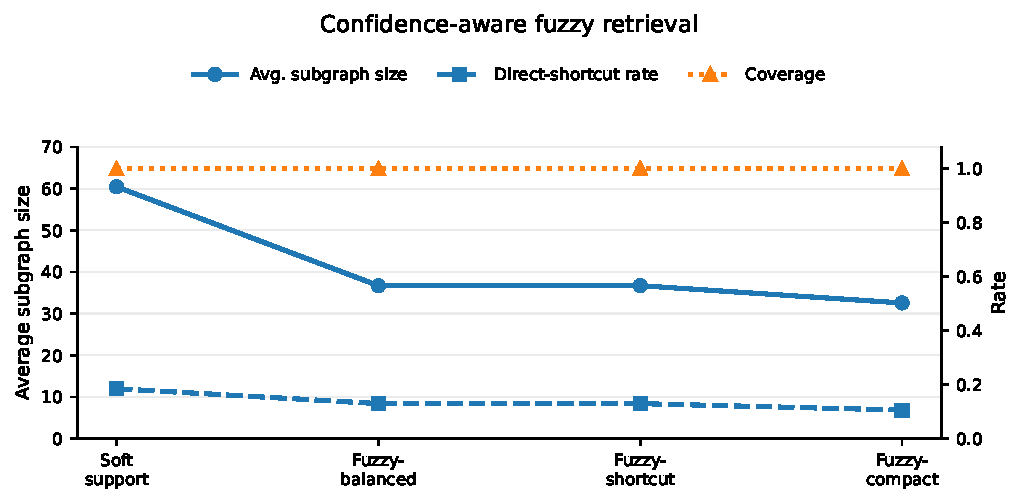
\includegraphics[width=\textwidth]{Fig3.pdf}
\caption{\textbf{Confidence-aware fuzzy retrieval selects the compact evidence package used after soft support.} The diagnostic plot compares the soft-support source graph with fuzzy retrieval variants in terms of average subgraph size, direct-shortcut exposure, and candidate coverage. Because fuzzy retrieval preserves the soft-support candidate order, the selected variant is chosen for graph efficiency and evidence cleanliness while maintaining Gold@20, MRR@20, and candidate coverage}
\label{fig:fuzzy}
\end{figure*}

\subsection{Graph-adapter-enhanced generation}

For each query, the prompt represents the query entity and all candidate entities with special placeholders. The graph enhancer replaces their placeholder embeddings with graph-aware embeddings. Each entity begins with a frozen structural embedding from the lightweight ranker. When a subgraph is available and sufficiently large, a relation-aware graph convolution updates node representations within the query-specific graph. The adapter then projects the concatenation of the global and locally updated embeddings to the hidden dimension of the LLM:
\begin{equation}
\mathbf{z}_e =
\mathrm{Adapter}
\left(
[\mathbf{h}^{\mathrm{global}}_e;\mathbf{h}^{\mathrm{local}}_e]
\right).
\label{eq:adapter}
\end{equation}
If an entity is absent from the retrieved subgraph, its local embedding is set to its global embedding. This fallback prevents missing graph evidence from producing an invalid representation and is consistent with the soft-evidence interpretation.

We fine-tune the LLM through LoRA~\citep{hulora} adapters while training the graph adapter and keeping the structural embeddings frozen. The prompt requires one candidate entity as the answer. Llama 3.2 3B is the primary language model for end-to-end evaluation.

% =========================================================
% 4. Results
% =========================================================

\section{Experimental Results}
\label{sec:results}

\subsection{Datasets and task setting}
\label{sec:study_datasets}

We represent each BKG as a directed, multirelational graph of biomedical entities and typed relations. Across all five datasets, drug-focused therapeutic completion is formulated as head prediction. Given a query tail $t_q$, the system ranks a drug or compound head for the incomplete triple $(?,r_q,t_q)$, where $r_q$ is a dataset-specific therapeutic or indication-style relation. \tabref{tab:dataset_summary} summarizes the target tasks, data splits, restricted candidate universes, and prepared training/evidence graphs. The graph statistics describe the evidence supplied to the graph-compatible pipeline after target triples assigned to validation or test were excluded; they are not the sizes of the unprocessed source KGs.

\begin{table*}[!t]
\caption{\textbf{Summary of the five biomedical evaluation datasets.} Train, validation, and test values count target-relation triples. Candidates are the size of the restricted drug or compound universe. Graph edges, entities, and relations describe the prepared training/evidence graph after validation and test target edges were excluded.}
\label{tab:dataset_summary}
\centering
{\fontsize{8.0pt}{8.8pt}\selectfont
\setlength{\tabcolsep}{2.2pt}
\renewcommand{\arraystretch}{1.08}
\begin{tabular*}{\textwidth}{@{\extracolsep{\fill}}llrrrrrrr@{}}
\toprule
Dataset & Target relation & Train & Valid & Test & Candidates & Graph edges & Entities & Relations \\
\midrule
PrimeKG & indication & 8,388 & 500 & 500 & 1,801 & 136,351 & 10,453 & 4 \\
PharmKG & $T$ proxy & 28,960 & 500 & 500 & 1,342 & 386,768 & 7,247 & 28 \\
Hetionet & CtD & 555 & 100 & 100 & 1,552 & 2,249,997 & 47,031 & 24 \\
DRKG & DrugBank treats & 3,968 & 500 & 500 & 1,542 & 187,962 & 13,918 & 85 \\
repoDB & approved indication & 5,677 & 500 & 500 & 1,519 & 90,804 & 8,818 & 63 \\
\bottomrule
\end{tabular*}}
\end{table*}

PrimeKG~\citep{chandak2023building} is the primary evaluation setting. We derived a drug-restricted indication benchmark and prepared an evidence graph with four relation families: indication, target, associated\_with, and protein--protein interaction. This combination supports both direct therapeutic context and mechanism-oriented drug--gene--disease paths. PharmKG~\citep{zheng2021pharmkg} provides a transfer setting with a larger relation vocabulary. Its relation $T$ is treated as a therapeutic-association proxy rather than a confirmed clinical-indication label, so results on this dataset indicate transfer across graph semantics rather than direct replication of the PrimeKG task.

Hetionet~\citep{himmelstein2017systematic} uses the compound-treats-disease relation CtD, with the candidate universe restricted to compounds. Its evidence graph is much larger than the other prepared graphs and has a distinct topology and relation vocabulary, providing a test of robustness to graph scale and structure. For DRKG~\citep{drkg2020}, we use the DrugBank~\citep{wishart2018drugbank} relation \texttt{DRUGBANK::treats::Compound:Disease} as the target. The controlled evidence graph combines selected compound--gene target relations, disease--gene relations, gene--gene relations, and auxiliary compound--disease relations rather than using every raw DRKG edge.

In repoDB~\citep{brown2017standard}, approved drug--indication pairs define positive target triples, whereas failed pairs are retained as diagnostic evidence. repoDB disease identifiers are UMLS~\citep{bodenreider2004unified} CUIs \rev{retained as local disease nodes.} The resulting graph combines approved target edges, failed-like diagnostic edges, and DRKG-derived compound--gene and gene--gene evidence. \rev{The DRKG evidence is linked to repoDB compounds through exact DrugBank identifiers, while unmatched compounds remain in the task. This partial alignment limits query-specific mechanistic paths, making repoDB useful for evaluating calibration with sparse evidence. Supplementary Section S11.1 describes normalization, identifier coverage, graph construction, and split checks.}

Together, the five settings vary in target semantics, candidate-universe size, graph density, relation diversity, and availability of mechanism-oriented support. These differences allow the evaluation to distinguish improvements that transfer across datasets from effects that depend on a particular graph topology or evidence family.

\subsection{Evaluation metrics}
\label{sec:evaluation_protocol}

All experiments use the same fixed top-20 protocol. Candidate lists for validation and test queries are generated before scoring, and a gold entity absent from a list receives the sentinel rank 21. We use $K=20$ because this is the candidate-list size accepted by the graph-LLM backbone. It is also small enough for candidate-constrained generation while supporting informative Hits@1/3/10 and Gold@20 analyses.

\begin{revisionblock}Because neither module changes candidate membership, a gold entity missing from the retrieved list remains unrecoverable. Candidate MRR therefore measures changes in ordering at fixed coverage, rather than retrieval over the full entity set. We then use the end-to-end metrics defined below to assess the ranking after LLM generation.\end{revisionblock}

Here, $Q$ denotes the set of evaluation queries; $y_q$ is the gold entity for query $q$; $C_q$ is its fixed candidate list; and $\mathrm{rank}_C(y_q)$ is the one-based position of the gold entity in that list. A present gold entity receives its top-20 position, whereas an absent gold receives rank 21. Reciprocal rank is \rev{calculated} as follows:
\begin{equation}
\mathrm{RR@20}(q)=
\begin{cases}
1/\mathrm{rank}_C(y_q), & \mathrm{rank}_C(y_q)\leq20,\\
0, & \mathrm{rank}_C(y_q)=21.
\end{cases}
\label{eq:rr}
\end{equation}
The candidate MRR is \rev{calculated} as follows:
\begin{equation}
\mathrm{MRR@20}=\frac{1}{|Q|}\sum_{q\in Q}\mathrm{RR@20}(q).
\label{eq:mrr}
\end{equation}
Hits@K and Gold@20 are \rev{calculated} as follows:
\begin{equation}
\mathrm{Hits@}K =
\frac{1}{|Q|}
\sum_{q\in Q}
\mathbb{I}\left[\mathrm{rank}_C(y_q)\leq K\right],
\quad K\in\{1,3,10\},
\label{eq:hits}
\end{equation}
\begin{equation}
\mathrm{Gold@20}
=
\frac{1}{|Q|}
\sum_{q\in Q}
\mathbb{I}[y_q\in C_q].
\label{eq:gold}
\end{equation}
Hits@1, Hits@3, and Hits@10 measure first-choice accuracy, early-rank utility, and broader candidate-list usefulness, respectively. We report Gold@20 separately because candidate coverage is a prerequisite for candidate-constrained generation.

For end-to-end evaluation, the LLM output is normalized and matched against the candidate names. Let $\hat{y}_q$ denote the normalized generated answer. \rev{A normalized answer matching the gold entity gives E2E rank 1}, whereas an absent gold entity gives E2E rank 21. When the generated answer is incorrect but occurs above the gold entity in the candidate list, the gold rank is unchanged. In all other cases, the gold rank is displaced by one position:
\begin{equation}
r_{\mathrm{e2e}}(q)=
\begin{cases}
1, & \hat{y}_q = y_q,\\
21, & y_q \notin C_q,\\
\mathrm{rank}_C(y_q), &
\begin{array}{l}
\hat{y}_q \in C_q,\\[-0.2em]
\mathrm{rank}_C(\hat{y}_q)<\mathrm{rank}_C(y_q),
\end{array}\\
\min(21,\mathrm{rank}_C(y_q)+1), & \mathrm{otherwise}.
\end{cases}
\label{eq:e2e_rank}
\end{equation}
The end-to-end reciprocal rank is \rev{calculated as follows}:
\begin{equation}
\mathrm{RR@20}_{\mathrm{e2e}}(q)=
\begin{cases}
1/r_{\mathrm{e2e}}(q), & r_{\mathrm{e2e}}(q)\leq20,\\
0, & r_{\mathrm{e2e}}(q)=21.
\end{cases}
\label{eq:e2e_rr}
\end{equation}
\rev{E2E MRR is the mean of these reciprocal ranks and thus reflects both the supplied candidate order and the generated answer. To keep the comparisons consistent, all module, calibration, and graph-selection experiments use the same deterministic generation and answer-matching protocol within each dataset. Supplementary Sections S12--S13 describe the downstream comparisons in detail.}

\subsection{Candidate stage comparison with structure baselines}

The first analysis evaluates candidate retrieval before LLM generation. This stage determines whether candidate-constrained generation can recover the gold drug. A gold entity outside the fixed top-20 list cannot be selected, while a gold entity near the tail remains difficult for both the model and a human reviewer to identify. \tabref{tab:candidate_baselines} therefore reports three complementary quantities. Gold@20 measures recoverability, MRR@20 measures gold position under the absent-gold rank-21 rule, and Hits@10 indicates whether the gold appears in the upper half of the list.

\begin{table*}[!t]
\caption{\textbf{Fixed top-20 candidate-ranking comparison across five biomedical datasets.} All values are test metrics under the same absent-gold rank-21 rule. Metrics marked with ($\uparrow$) are better when larger. Bold marks the best value for each dataset and metric. \softfuse{} is the main graph-compatible row and should be interpreted as an evidence-calibrated \drkgc{}-style source, not as a universal replacement for the strongest structure-only candidate generator.}
\label{tab:candidate_baselines}
\centering
{\fontsize{8.1pt}{8.9pt}\selectfont
\setlength{\tabcolsep}{2.8pt}
\renewcommand{\arraystretch}{1.07}
\begin{tabular*}{\textwidth}{@{\extracolsep{\fill}}llccccc@{}}
\toprule
Model & Metric & PrimeKG & PharmKG & Hetionet & DRKG & repoDB \\
\midrule
\multirow{3}{*}{TransE}
& Gold@20 ($\uparrow$) & 0.104 & 0.060 & 0.270 & 0.270 & 0.248 \\
& MRR@20 ($\uparrow$) & 0.022 & 0.009 & 0.046 & 0.055 & 0.053 \\
& Hits@10 ($\uparrow$) & 0.072 & 0.028 & 0.150 & 0.160 & 0.130 \\
\midrule
\multirow{3}{*}{DistMult}
& Gold@20 ($\uparrow$) & 0.434 & \textbf{0.102} & 0.390 & \textbf{0.432} & 0.482 \\
& MRR@20 ($\uparrow$) & 0.089 & 0.017 & 0.072 & \textbf{0.100} & \textbf{0.104} \\
& Hits@10 ($\uparrow$) & 0.264 & 0.038 & \textbf{0.290} & \textbf{0.276} & \textbf{0.320} \\
\midrule
\multirow{3}{*}{ComplEx}
& Gold@20 ($\uparrow$) & \textbf{0.574} & 0.066 & \textbf{0.440} & 0.406 & \textbf{0.502} \\
& MRR@20 ($\uparrow$) & 0.125 & 0.009 & 0.090 & 0.086 & 0.084 \\
& Hits@10 ($\uparrow$) & \textbf{0.384} & 0.036 & 0.250 & 0.260 & 0.312 \\
\midrule
\multirow{3}{*}{RotatE}
& Gold@20 ($\uparrow$) & 0.134 & 0.024 & 0.200 & 0.182 & 0.202 \\
& MRR@20 ($\uparrow$) & 0.033 & 0.002 & 0.043 & 0.024 & 0.022 \\
& Hits@10 ($\uparrow$) & 0.074 & 0.004 & 0.120 & 0.098 & 0.100 \\
\midrule
\multirow{3}{*}{R-GCN}
& Gold@20 ($\uparrow$) & 0.220 & 0.092 & \textbf{0.440} & 0.200 & 0.214 \\
& MRR@20 ($\uparrow$) & 0.060 & 0.020 & 0.099 & 0.043 & 0.048 \\
& Hits@10 ($\uparrow$) & 0.186 & 0.046 & 0.220 & 0.120 & 0.128 \\
\midrule
\multirow{3}{*}{HRGAT}
& Gold@20 ($\uparrow$) & 0.212 & 0.094 & 0.410 & 0.204 & 0.222 \\
& MRR@20 ($\uparrow$) & 0.033 & 0.019 & \textbf{0.101} & 0.042 & 0.052 \\
& Hits@10 ($\uparrow$) & 0.128 & 0.044 & \textbf{0.290} & 0.134 & 0.146 \\
\midrule
\multirow{3}{*}{\drkgc{}-style source}
& Gold@20 ($\uparrow$) & 0.240 & 0.092 & \textbf{0.440} & 0.200 & 0.214 \\
& MRR@20 ($\uparrow$) & 0.065 & 0.020 & 0.099 & 0.043 & 0.048 \\
& Hits@10 ($\uparrow$) & 0.192 & 0.046 & 0.220 & 0.120 & 0.128 \\
\midrule
\multirow{3}{*}{\softfuse{}}
& Gold@20 ($\uparrow$) & 0.240 & 0.092 & \textbf{0.440} & 0.200 & 0.214 \\
& MRR@20 ($\uparrow$) & \textbf{0.125} & \textbf{0.028} & 0.095 & 0.047 & 0.048 \\
& Hits@10 ($\uparrow$) & 0.222 & \textbf{0.068} & 0.280 & 0.142 & 0.128 \\
\bottomrule
\end{tabular*}}
\end{table*}

\afterpage{%
\begin{table*}[!t]
\caption{\textbf{End-to-end module comparison for the graph-LLM pipeline.} Gold@20, candidate MRR@20, and E2E MRR@20 are higher-is-better metrics ($\uparrow$), whereas average graph size is lower-is-better ($\downarrow$). E2E MRR@20 uses Llama 3.2 3B candidate-constrained generation with the adjusted-rank rule defined in Section~\ref{sec:evaluation_protocol}. Bold marks the best row for each dataset and metric where the comparison is meaningful.}
\label{tab:module_results}
\centering
{\fontsize{8.1pt}{8.9pt}\selectfont
\setlength{\tabcolsep}{3.4pt}
\renewcommand{\arraystretch}{1.08}
\begin{tabular*}{\textwidth}{@{\extracolsep{\fill}}llccccc@{}}
\toprule
Row & Metric & PrimeKG & PharmKG & Hetionet & DRKG & repoDB \\
\midrule
\multirow{4}{*}{\drkgc{}-style source}
& Gold@20 ($\uparrow$) & 0.240 & 0.092 & 0.440 & 0.200 & 0.214 \\
& Candidate MRR@20 ($\uparrow$) & 0.0646 & 0.0205 & \textbf{0.0994} & 0.0432 & \textbf{0.0481} \\
& E2E MRR@20 ($\uparrow$) & \revisioncell{0.0477} & 0.0156 & \revisioncell{0.0819} & \revisioncell{0.0410} & \revisioncell{0.0366} \\
& Avg. graph ($\downarrow$) & 59.93 & 100.00 & 80.00 & 100.00 & 100.00 \\
\midrule
\multirow{4}{*}{Soft support}
& Gold@20 ($\uparrow$) & 0.240 & 0.092 & 0.440 & 0.200 & 0.214 \\
& Candidate MRR@20 ($\uparrow$) & \textbf{0.1253} & \textbf{0.0282} & 0.0954 & \textbf{0.0466} & 0.0481 \\
& E2E MRR@20 ($\uparrow$) & \textbf{0.0747} & \revisioncell{0.0207} & \revisioncell{\textbf{0.1001}} & \revisioncell{\textbf{0.0463}} & \revisioncell{0.0366} \\
& Avg. graph ($\downarrow$) & 59.93 & 100.00 & 80.00 & 100.00 & 100.00 \\
\midrule
\multirow{4}{*}{Fuzzy retrieval}
& Gold@20 ($\uparrow$) & 0.240 & 0.092 & 0.440 & 0.200 & 0.214 \\
& Candidate MRR@20 ($\uparrow$) & \textbf{0.1253} & \textbf{0.0282} & 0.0954 & \textbf{0.0466} & \textbf{0.0481} \\
& E2E MRR@20 ($\uparrow$) & \textbf{0.0747} & \textbf{0.0210} & \revisioncell{\textbf{0.1001}} & \revisioncell{\textbf{0.0463}} & \revisioncell{\textbf{0.0378}} \\
& Avg. graph ($\downarrow$) & \textbf{32.34} & \textbf{55.00} & \textbf{44.00} & \textbf{55.00} & \textbf{55.00} \\
\bottomrule
\end{tabular*}}
\end{table*}
}

The table contains two types of rows. The standalone structure-only baselines provide reference candidate-retrieval performance for conventional embedding and graph models. The \drkgc{}-style source and \softfuse{} rows are graph-compatible: in addition to ranking candidates, they must provide identifiers, embeddings, and query-specific source subgraphs for the graph adapter. Both graph-compatible rows use the same lightweight R-GCN-compatible source. Their difference therefore reflects evidence calibration rather than replacement of the upstream retriever.

PrimeKG provides the clearest candidate-stage result. \softfuse{} increases MRR@20 from 0.065 to 0.125 while Gold@20 remains 0.240, showing that soft support reorders recoverable candidates rather than expanding the set. PharmKG follows the same direction in the transfer setting: MRR@20 rises from 0.020 to 0.028 and Hits@10 from 0.046 to 0.068, with Gold@20 unchanged at 0.092. DRKG shows a smaller positive MRR@20 change, from 0.043 to 0.047. Hetionet is mixed. Gold@20 remains 0.440 and Hits@10 increases from 0.220 to 0.280, but MRR@20 decreases from 0.099 to 0.095. Soft support therefore improves some upper-half placements while moving a small number of first-rank cases downward. repoDB is neutral at the candidate stage, consistent with its local UMLS disease nodes and sparse query-specific mechanistic support.

The standalone results provide context for these changes. ComplEx achieves the highest PrimeKG Gold@20; HRGAT and R-GCN are strong on Hetionet; and DistMult has the highest candidate MRR@20 on DRKG and repoDB. \softfuse{} should therefore not be interpreted as a replacement for the strongest structure-only retriever. Its specific role is to calibrate the graph-compatible candidate package passed to the graph-LLM pipeline. The next analysis tests whether candidate calibration and evidence selection are reflected in end-to-end behavior.

\subsection{End-to-end graph-LLM pipeline comparison}

\tabref{tab:module_results} compares the three graph-compatible pipeline rows after candidate-constrained generation: the raw \drkgc{}-style source, the soft-support row, and the confidence-aware fuzzy retrieval row. This system-level comparison reflects both inputs available to the downstream model: an ordered candidate list and a query-specific graph package delivered through the adapter. It also isolates the proposed modules. Soft support changes candidate order, whereas fuzzy retrieval preserves that order and changes the evidence graph.


\begin{revisionblock}
On PrimeKG, the candidate-ranking improvement is accompanied by an increase in E2E MRR@20 from 0.0477 to 0.0747 after soft support. Fuzzy retrieval preserves this value while reducing the average input from 59.93 to 32.34 edge occurrences, partly through duplicate removal. PharmKG shows a similar pattern: E2E MRR@20 increases from 0.0156 for the raw source to 0.0207 with soft support and 0.0210 with fuzzy retrieval, while the graph shrinks from 100 to 55 triples.
\end{revisionblock}



\begin{revisionblock}
On Hetionet, soft support increases E2E MRR@20 from 0.0819 to 0.1001 despite a slightly lower candidate MRR than the raw source. Fuzzy retrieval retains 0.1001 while reducing the graph from 80 to 44 triples. On DRKG, E2E MRR@20 similarly increases from 0.0410 to 0.0463 after soft support and remains at 0.0463 after compression. On repoDB, where the original candidate order is retained, fuzzy retrieval raises E2E MRR@20 from 0.0366 to 0.0378 while reducing the graph from 100 to 55 triples. These comparisons show that a smaller evidence package can retain E2E ranking performance.
\end{revisionblock}


These findings support two related but distinct conclusions. Soft support is most useful when the prepared graph contains query-specific features that distinguish candidates, as on PrimeKG and PharmKG and, more modestly, DRKG. Its effect is weaker when support is sparse or graph topology differs, as in repoDB and parts of Hetionet. Fuzzy retrieval primarily improves evidence efficiency. By design, it preserves the candidate MRR of its input row, while reducing graph size by approximately 45\% in every fuzzy setting. The graph adapter consequently receives a smaller and more inspectable context, and retained evidence is easier to audit. The repoDB result indicates relevance to a clinical benchmark rather than prospective clinical validation: the dataset includes approved pairs and failed-like evidence, but its local UMLS disease nodes limit query-specific mechanistic support.

% =========================================================
% Results case studies
% =========================================================

% Revised 2026-11-11: integrated Results, prose table introductions, and adjacent Tables 4--5.
\subsection{\rev{Automatic calibration and coefficient transfer}}
\label{sec:calibration_results}
\begin{revisionblock}
To assess the effect of coefficient choice on soft support, we compare equal, learned, and leave-one-dataset-out (LODO) weights for a common five-feature scorer. Learned weights use target-dataset validation data with query-group cross-validation, whereas LODO weights use the other four datasets without target calibration labels. All settings preserve candidate membership. \tabref{tab:calibration_main} compares their candidate MRR on the complete test splits with that of the original soft-support formula.

% Keep the two summary tables together, without intervening prose.
\end{revisionblock}
\begin{tableorg}[!t]
\begin{revisionblock}
\par\noindent\begin{minipage}{\linewidth}

\centering\small
\captionof{table}{\textbf{Candidate calibration on the complete test splits.} MRR@20 is computed over all rows, with zero reciprocal rank for absent gold entities. Shared equal, learned, and LODO use the same features; comparison with the original soft-support formula also changes features. LODO is coefficient transfer without target calibration labels. Bold marks the highest displayed MRR in each row, including ties.}
\label{tab:calibration_main}
\setlength{\tabcolsep}{6pt}
\begin{tabular}{lrrrrr}
\toprule
Dataset & Gold@20 & Original soft & Shared equal & Learned & LODO \\
\midrule
PrimeKG & 0.240 & 0.12533 & 0.12519 & 0.12533 & \textbf{0.12610} \\
PharmKG & 0.092 & 0.02816 & \textbf{0.03188} & \textbf{0.03188} & 0.03186 \\
Hetionet & 0.440 & 0.09544 & 0.10127 & \textbf{0.11528} & 0.11358 \\
DRKG & 0.200 & 0.04656 & \textbf{0.06143} & 0.06050 & 0.05861 \\
repoDB & 0.214 & 0.04811 & 0.05737 & \textbf{0.06490} & \textbf{0.06490} \\
\bottomrule
\end{tabular}


\end{minipage}\par\noindent\rule{0pt}{12pt}\par
\par\noindent\begin{minipage}{\linewidth}

\centering\small
\captionof{table}{\textbf{Three-hop reachability at matched unique-edge budgets.} Reachability is the per-row fraction of source-reachable candidates still reachable within three edges. $N$ counts evaluation rows with at least one source-reachable candidate. Random is mean $\pm$ standard deviation over five seeds. Fuzzy retrieval preserves incident evidence for every source-covered candidate (retention 1.0000 on all datasets). Bold marks the highest reachability in each row.}
\label{tab:retention_main}
\setlength{\tabcolsep}{5pt}
\begin{tabular}{lrrrrr}
\toprule
Dataset & $N$ & Fuzzy & Random & Shortest paths & Shortest coverage \\
\midrule
PrimeKG & 488 & 0.7737 & $0.7760\pm0.0038$ & \textbf{0.9985} & 0.9993 \\
PharmKG & 500 & 0.9010 & $0.4423\pm0.0064$ & \textbf{1.0000} & 1.0000 \\
Hetionet & 90 & 0.4835 & $0.4848\pm0.0428$ & \textbf{1.0000} & 0.8514 \\
DRKG & 386 & 0.8921 & $0.5043\pm0.0170$ & \textbf{1.0000} & 0.8199 \\
repoDB & 297 & 0.9546 & $0.5465\pm0.0241$ & \textbf{1.0000} & 0.8971 \\
\bottomrule
\end{tabular}


\end{minipage}\par\medskip
\end{revisionblock}
\end{tableorg}
\begin{revisionblock}

Learned weights improve candidate MRR over the original formula on four datasets and match it on PrimeKG, while LODO weights yield higher point estimates on all five. However, equal weights also improve four datasets, indicating that the shared feature set contributes to these gains. The learned-minus-equal comparison isolates the effect of learning the weights: the gain on repoDB is 0.00754, with an exploratory query-cluster 95\% interval of [0.00040, 0.01518], whereas the other four intervals include zero.

To examine coefficient choice in fuzzy retrieval as well, we evaluate validation-based selection among 12 edge-scoring coefficient vectors while fixing candidate order and graph budget. Supplementary Section S12 and Tables S16--S24 report these results together with the fitting procedures, coefficient-transfer tests, sensitivity analyses, and downstream comparisons.
\end{revisionblock}

\subsection{\rev{Information retention and alternative graph selection}}
\label{sec:retention_results}
\begin{revisionblock}
To examine which information is retained during graph compression, we compare fuzzy retrieval with alternative selectors using the same number of unique edges per query and the same candidate identities and order. The alternatives include random and coverage-constrained random sampling, native-score and degree selection, breadth-first search, personalized PageRank, shortest paths, and relation-stratified selection. \tabref{tab:retention_main} summarizes three-hop query--candidate reachability and candidate-incidence coverage for fuzzy retrieval and two representative controls.

Fuzzy retrieval preserves incident evidence for every candidate covered by the source graph. It also retains more three-hop reachability than uniform random selection on PharmKG, DRKG, and repoDB, with similar values on PrimeKG and Hetionet. Shortest-path selection preserves nearly all source connectivity, but covers fewer candidates on Hetionet, DRKG, and repoDB. This contrast shows that retaining evidence for each candidate and preserving its paths to the query are distinct objectives.

Supplementary Section S13, Tables S25--S29, and Figs.~S4--S6 provide the full selector comparison and analyses of labeled paths, encoder representations, downstream behavior, and graph budgets. They also separate reductions due to duplicate removal from losses of unique triples. Together, these results show that fuzzy retrieval preserves candidate coverage during compression, while path retention depends on graph topology.
\end{revisionblock}


\subsection{Case studies}

The case studies examine whether the numerical changes in \tabref{tab:module_results} correspond to evidence changes that a biomedical reader can inspect. A correct graph-augmented LLM answer may arise in several ways: the candidate generator may already rank the gold drug highly, the LLM may select an already high-ranked candidate, or evidence calibration may promote a recoverable but low-ranked candidate. We therefore examine representative PrimeKG examples in terms of rank change, graph-size reduction, retained internal evidence, and external biomedical plausibility.

\tabref{tab:case_rank} groups the cases into three diagnostic categories. Improved cases test whether soft support promotes recoverable, low-ranked gold drugs to more visible positions. Sparse cases test whether graded scoring avoids brittle hard filtering when graph support is incomplete. Cleaner cases assess fuzzy graph reduction when candidate ranks change little. This taxonomy follows the division of labor within \softfuse{}: soft support targets candidate order, whereas fuzzy retrieval targets evidence efficiency. \figref{fig:case} visualizes the two principal examples, and \tabref{tab:case_evidence} reports external evidence identifiers for model-selected candidates.

\begin{table*}[!tp]
\centering
\caption{\textbf{PrimeKG diagnostic cases of candidate promotion and evidence compression.} Base and Soft denote gold-drug ranks before and after soft-support reranking; Removed is the number of triples discarded by fuzzy retrieval. These cases audit rank and evidence changes rather than provide treatment recommendations.}
\label{tab:case_rank}
\makebox[\textwidth][c]{%
{\fontsize{8.4pt}{9.25pt}\selectfont
\setlength{\tabcolsep}{3.2pt}
\renewcommand{\arraystretch}{1.12}
\begin{tabularx}{0.985\textwidth}{@{}>{\raggedright\arraybackslash}p{1.45cm}>{\raggedright\arraybackslash}p{4.0cm}ccc>{\raggedright\arraybackslash}X@{}}
\toprule
Bucket & Query / gold drug & Base & Soft & Removed & Interpretation \\
\midrule
Improved & lymphosarcoma / Vincristine & 16 & 2 & 20 & Soft support promotes an evidence-connected antineoplastic candidate, and fuzzy retrieval preserves the improved order. \\
Improved & lymphoma / Vincristine & 17 & 3 & 20 & The gold drug is promoted from the tail under related lymphoma terminology. \\
Improved & rheumatoid arthritis / Methotrexate & 19 & 8 & 23 & The benchmark gold drug moves upward, showing why Gold@20 and MRR@20 should be reported together. \\
Sparse & seborrheic dermatitis / Cortisone acetate & 1 & 1 & 26 & Soft scoring avoids strict filtering when graph evidence is incomplete. \\
Cleaner & chronic otitis media / Norfloxacin & 4 & 4 & 38 & Candidate order is preserved while the graph package is substantially reduced. \\
Cleaner & cholera / Fusidic acid & 1 & 1 & 33 & Fuzzy retrieval removes redundant or shortcut-heavy evidence. \\
Cleaner & botulism / Ofloxacin & 12 & 10 & 30 & Candidate ordering is mostly preserved with a cleaner evidence graph. \\
\bottomrule
\end{tabularx}}}
\end{table*}

\begin{figure*}[!tp]
\centering
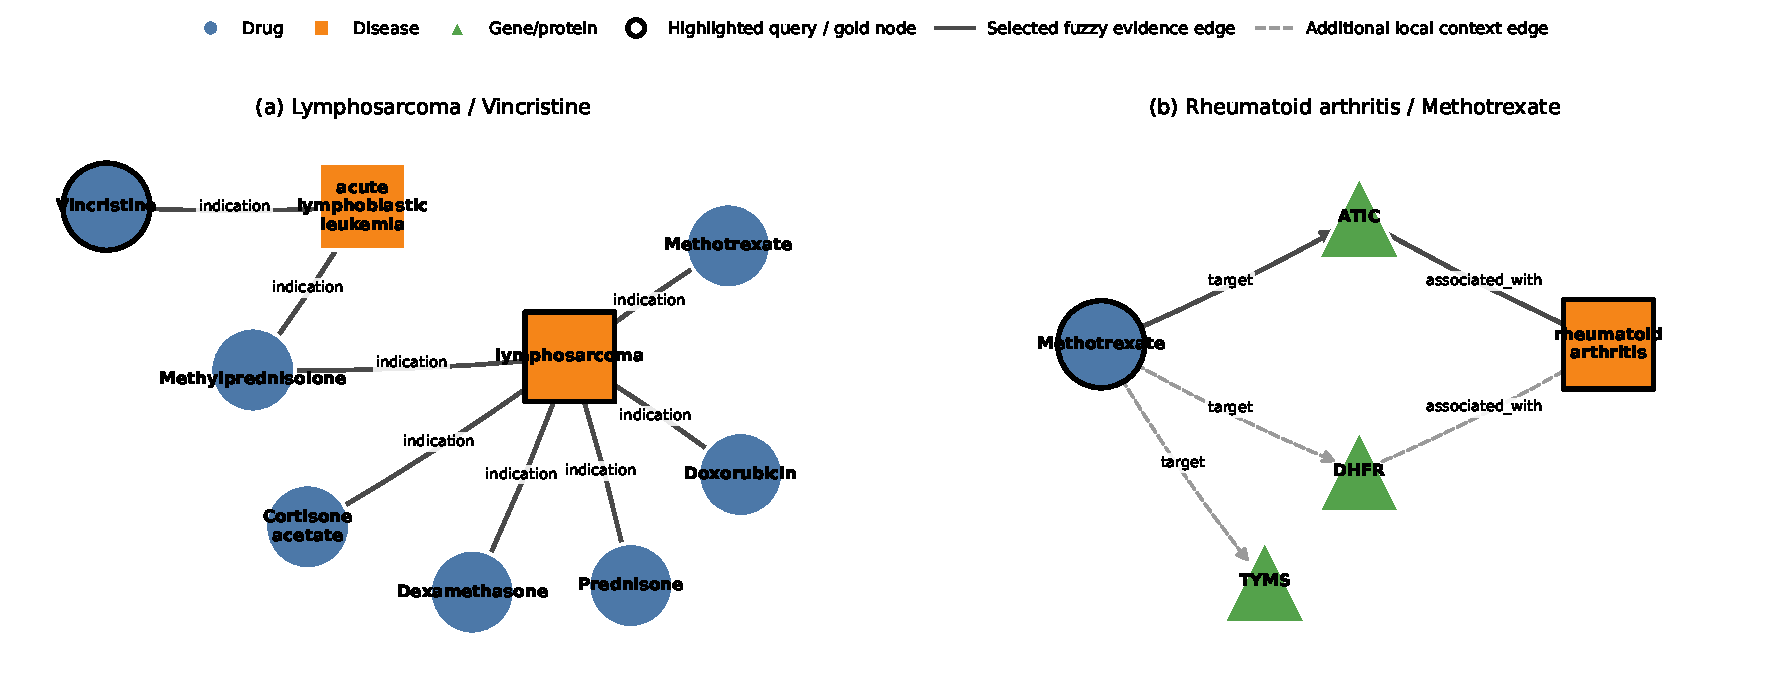
\includegraphics[width=\textwidth]{Fig4.pdf}
\caption{\textbf{Case-study evidence graphs for lymphosarcoma / Vincristine and rheumatoid arthritis / Methotrexate.} Circles denote drugs, squares denote diseases, and triangles denote genes or proteins. Thick solid edges show evidence selected by fuzzy retrieval, whereas dashed edges show additional local context. Black outlines identify the query disease and gold drug, making rank changes and retained evidence auditable}
\label{fig:case}
\end{figure*}

\begin{table*}[!tp]
\caption{\textbf{Internal graph evidence and external plausibility evidence for case-study candidates.} Candidate drugs come from the corresponding \softfuse{} ranked lists, and internal evidence is extracted from the fuzzy-retrieved graph. The external evidence column provides a literature citation and PubMed identifier for candidate--disease plausibility or related clinical context. These references support plausibility checking and auditability, not prospective clinical validation, graph-edge provenance, or treatment recommendations.}
\label{tab:case_evidence}
\centering
{\fontsize{8.4pt}{9.25pt}\selectfont
\setlength{\tabcolsep}{2.4pt}
\renewcommand{\arraystretch}{1.13}
\begin{tabularx}{0.995\textwidth}{@{}>{\raggedright\arraybackslash}p{0.172\textwidth}>{\raggedright\arraybackslash}p{0.165\textwidth}>{\raggedright\arraybackslash}p{0.115\textwidth}>{\raggedright\arraybackslash}X>{\raggedright\arraybackslash}p{0.178\textwidth}@{}}
\toprule
Case disease & Candidate drug & Model rank / band & Internal \softfuse{} evidence & External plausibility evidence \\
\midrule
Lymphosarcoma & Prednisolone & Rank 1 / top & Prednisolone -- indication -- mycosis fungoides and variants & \citep{sweetenham1993pacet}; \pmid{8422281} \\
Lymphosarcoma & Vincristine & Rank 2 / top & Vincristine -- indication -- acute lymphoblastic leukemia & \citep{bagley1972lymphosarcoma}; \pmid{5066691} \\
Lymphosarcoma & Dexamethasone & Rank 5 / top & Dexamethasone -- indication -- lymphosarcoma; reverse direct edge retained & \citep{mclaughlin1994fnd}; \pmid{8120556} \\
Lymphosarcoma & Doxorubicin & Rank 12 / tail & Doxorubicin -- indication -- lymphosarcoma & \citep{fisher1993chop}; \pmid{7680764} \\
Lymphosarcoma & Bleomycin & Rank 15 / tail & Bleomycin -- indication -- lymphosarcoma & \citep{bayer1992bleomycin}; \pmid{1384144} \\
\midrule
Rheumatoid arthritis & Methotrexate & Rank 8 / mid & Methotrexate -- target -- ATIC; ATIC -- associated\_with -- rheumatoid arthritis & \citep{fraenkel20212021}; \pmid{34101387} \\
Rheumatoid arthritis & Dexamethasone & Rank 11 / tail & Dexamethasone -- indication -- rheumatoid arthritis & \citep{jick1965dexamethasone}; \pmid{4158821} \\
Rheumatoid arthritis & Hydrocortisone & Rank 13 / tail & Hydrocortisone -- indication -- rheumatoid arthritis & \citep{blyth1994rheumatoidknee}; \pmid{8173851} \\
Rheumatoid arthritis & Prednisolone & Rank 16 / tail & Prednisolone -- indication -- rheumatoid arthritis & \citep{boers2022gloria}; \pmid{35641125} \\
Rheumatoid arthritis & Prednisone & Rank 18 / tail & Prednisone -- indication -- rheumatoid arthritis & \citep{buttgereit2008capra1}; \pmid{18207016} \\
\bottomrule
\end{tabularx}}
\renewcommand{\arraystretch}{1.0}
\end{table*}

The first principal case is lymphosarcoma / vincristine. Vincristine occurs in the raw \drkgc{}-style top-20 list but only at rank 16. Soft support promotes it to rank 2, after which fuzzy retrieval preserves the improved order while reducing the evidence subgraph from 45 to 25 triples. This example is informative because ``lymphosarcoma'' is a historical lymphoma-related term. \figref{fig:case}(a) shows that fuzzy retrieval retains the promoted vincristine context and additional lymphoma-relevant local evidence while removing redundant triples.

The second principal case is rheumatoid arthritis / methotrexate. Clinical guidance, labeling, and clinical studies identify methotrexate as an established rheumatoid arthritis therapy \citep{fraenkel20212021,weinblatt1994methotrexate,van2007efficacy}. The raw candidate generator retrieves methotrexate at rank 19, a weak position for candidate-constrained generation and manual review. Soft support raises it to rank 8, and fuzzy retrieval preserves that rank while reducing the graph from 52 to 29 triples. \figref{fig:case}(b) retains the mechanistic Methotrexate--ATIC--rheumatoid arthritis path together with additional target and association context. The example illustrates why Gold@20 and MRR@20 should be considered together: the raw list contains the gold drug, but its position limits practical utility.

The external evidence in \tabref{tab:case_evidence} provides a plausibility check for model-selected candidates rather than provenance for every internal graph edge. In the lymphosarcoma case, the table includes the promoted gold drug Vincristine and other lymphoma-context candidates ranked by the model. In the rheumatoid arthritis case, methotrexate is the gold candidate, whereas the listed steroids represent adjunctive anti-inflammatory context. The candidates are not claimed to be therapeutically equivalent.

The remaining cases illustrate complementary behavior. Cortisone acetate remains at rank 1 for seborrheic dermatitis and shows why binary filtering can be risky when graph support is incomplete. The chronic otitis media / norfloxacin, cholera / fusidic acid, and botulism / ofloxacin examples show that fuzzy retrieval can remove redundant or shortcut-heavy triples while preserving candidate order. Because graph proximity does not itself establish therapeutic appropriateness, all cases require cautious biomedical interpretation. Their purpose is to show that \softfuse{} makes rank and evidence changes auditable, not to provide clinical validation.

%\subsection{Web application}
%
%We provide a public web application for interactive inspection of the \softfuse{} pipeline at \url{https://inosuke710-softfuse-kgc-demo.hf.space/}. It uses precomputed artifacts and allows users to select a dataset, split, disease or query case, and top-\(k\) value before viewing the Overview, Soft Support, and Fuzzy Retrieval tabs. Across tabs, the interface links a selected case to summary metrics, candidate-level support features, rank changes, and retained evidence edges. Users can therefore trace a reranking or graph-compression result to the final evidence package. Online Resource 1 provides screenshots and tab-level instructions under \textit{The Web Application}.

% =========================================================
% 5. Discussion
% =========================================================

\section{Discussion}
\label{sec:discussion}

The results support soft, confidence-aware evidence modeling for biomedical graph-augmented LLM completion. More specifically, they show that candidate ordering and graph-evidence selection are separate problems. Soft support can improve ranking when the available evidence differentiates candidates, whereas fuzzy retrieval can reduce graph size without changing the candidate list. This distinction matters in biomedical informatics because ranking performance, evidence efficiency, and interpretability all affect the usefulness of a graph-LLM pipeline.


Evaluation across five datasets shows that the benefit of soft support depends on the evidence available for each query. \rev{The supplementary calibration study shows that learned and transferred weights offer alternatives to manual coefficient assignment, although their gains depend on the dataset and scoring features. For fuzzy retrieval, the graph-selection comparisons reveal a related dependence on the evidence objective: preserving an incident edge for each candidate does not necessarily preserve its paths to the query. Shortest-path selection retains more of this connectivity, whereas fuzzy retrieval maintains broader candidate coverage. These findings clarify the trade-offs involved in adapting the two modules to a particular dataset.}



The structure-only comparisons further define the scope of the contribution. R-GCN serves as the lightweight source because it matches the \drkgc{} graph-adapter interface and provides relation-aware local embeddings for the subgraph encoder. It is not assumed to be the strongest standalone candidate generator. The calibrated graph-compatible row is strongest or among the strongest in candidate MRR on PrimeKG and PharmKG, whereas HRGAT or DistMult performs better on Hetionet, DRKG, and repoDB. These results indicate the limitation imposed by the selected source but also illustrate the modularity of \softfuse{}. A future implementation could replace R-GCN with a stronger structural or hybrid retriever that exposes compatible entity embeddings, candidate lists, and query-specific evidence graphs.


repoDB is a clinically relevant external benchmark rather than clinical validation. Its approved drug--indication pairs and failed-like diagnostic evidence are useful for evaluation, but its local UMLS disease nodes do not map directly to the reused DRKG disease namespace. \rev{Despite this limited alignment, fuzzy retrieval reduces the average evidence graph from 100 to 55 triples while preserving candidate order. Learned calibration also improves candidate ranking over equal weights, suggesting that the shared structural features retain useful scoring information even in this sparse setting.}



The case studies make these behaviors more interpretable, but they require careful biomedical framing. The lymphosarcoma / vincristine example combines a large rank improvement with retained lymphoma-related evidence. The rheumatoid arthritis / methotrexate example combines a rank improvement with guideline, labeling, clinical-study, and graph-path context. These examples demonstrate candidate reranking and evidence packaging rather than clinical validity. \softfuse{} should therefore be used for prioritization, hypothesis generation, and evidence review. It does not replace clinical judgment, pharmacological assessment, or experimental validation.


\begin{revisionblock}
The current study has several limitations. Soft support depends on the available evidence and cannot recover drugs outside the retrieved top-20 list. Fuzzy retrieval uses predefined scoring features and graph budgets, so preserving candidate coverage does not ensure preservation of query--candidate paths. Learned coefficients reduce manual tuning, but transfer within prepared benchmarks does not establish generalization to unseen graphs or diseases. Differences in relation semantics and entity alignment further constrain cross-dataset comparisons. The evaluation is retrospective, and the qualitative case studies require domain-expert review.
\end{revisionblock}




\begin{revisionblock}
The spatial--spectral and frequency-domain models reviewed in Section~\ref{sec:related} suggest one way to address the reliance on predefined evidence features~\citep{zhu2026spatialspectral,zhu2026fdmsgl}. Learning molecular, interaction, and pathway representations jointly with fusion weights could enrich candidate scoring. These representations could also guide graph selection under an edge budget, with an explicit objective for retaining relevant paths. Such an extension would require consistent entity alignment and held-out evaluation.
\end{revisionblock}

% =========================================================
% 6. Conclusion
% =========================================================

\section{Conclusion}
\label{sec:conclusion}


\begin{revisionblock}
We presented \softfuse{}, an evidence-calibration framework with two complementary modules for biomedical graph-augmented LLM completion. Soft support first reranks retrieved drug candidates using graded evidence, with penalties for shortcuts and contradictions. Confidence-aware fuzzy retrieval then selects a compact evidence graph while preserving the chosen candidate order. Across five biomedical datasets, these modules improve candidate ranking in several settings and reduce graph size while retaining comparable E2E ranking performance. Their benefits depend on the available evidence, as further clarified by the calibration and retention analyses. The case studies and web interface make these effects inspectable through candidate scores, rank changes, and retained graph evidence.
\end{revisionblock}


Future work will pursue several directions. First, we will integrate stronger structural and hybrid candidate retrievers to improve candidate coverage while retaining compatibility with the graph-adapter interface. \rev{Second, we will extend the evaluated linear calibration to uncertainty-aware multi-source fusion and query-adaptive graph budgets.} Third, we will strengthen cross-dataset entity and ontology alignment, particularly between repoDB UMLS concepts and mechanistic graph namespaces, and extend the evaluation to additional therapeutic relations. Fourth, learned evidence retrievers will be studied to balance graph compression against end-to-end performance across different graph topologies. Finally, temporal evaluation, broader language-model comparisons, and domain-expert assessment will be used to examine whether the retained evidence remains robust, mechanistically informative, and clinically plausible.

% =========================================================
% Supplementary information and declarations
% =========================================================

\backmatter

\bmhead{Supplementary Information}

Additional details are provided in the Supplementary Material. The opening \textit{The Web Application} section describes the public demo, screenshots, and tab-level usage notes. We provide a public web application for interactive inspection of the \softfuse{} pipeline at \url{https://inosuke710-softfuse-kgc-demo.hf.space/}. It uses precomputed artifacts and allows users to select a dataset, split, disease or query case, and top-\(k\) value before viewing the Overview, Soft Support, and Fuzzy Retrieval tabs. Across tabs, the interface links a selected case to summary metrics, candidate-level support features, rank changes, and retained evidence edges. Users can therefore trace a reranking or graph-compression result to the final evidence package. Sections S1--S3 report feature selection, weight assignment, frozen soft-support coefficients, fuzzy edge-scoring weights, and graph-budget checks. Sections S4--S6 provide the inference algorithm, graph-LLM settings, prompt and retrieval-rule templates, and PrimeKG formula variants. Sections S7--S9 report LLM comparisons, decoding checks, ablation, sensitivity, robustness, and the fuzzy encoder probe. Sections S10--S11 provide structure-only baseline training settings, dataset preprocessing, and leakage checks. \rev{Section S12 provides automatic calibration, coefficient transfer, sensitivity analyses, and downstream comparisons. Section S13 reports alternative subgraph selectors, information retention, and budget analyses.} Tables S1--S15 contain the corresponding configuration and diagnostic summaries. \rev{Tables S16--S24 summarize the calibration experiments, and Tables S25--S29 report the subgraph-selection comparisons. Figs. S1--S3 illustrate the web application, while Figs. S4--S6 present retention, budget, and representation analyses.}

%We provide a public web application for interactive inspection of the \softfuse{} pipeline at \url{https://inosuke710-softfuse-kgc-demo.hf.space/}. It uses precomputed artifacts and allows users to select a dataset, split, disease or query case, and top-\(k\) value before viewing the Overview, Soft Support, and Fuzzy Retrieval tabs. Across tabs, the interface links a selected case to summary metrics, candidate-level support features, rank changes, and retained evidence edges. Users can therefore trace a reranking or graph-compression result to the final evidence package. 
%Online Resource 1 provides screenshots and tab-level instructions under \textit{The Web Application}.

%Online Resource 1 (ESM\_1.pdf). Supplementary methods, dataset-specific coefficients, retrieval budgets, implementation settings, model comparisons, ablation and robustness analyses, preprocessing and leakage checks, and screenshots and instructions for the \softfuse{} web application.

%\bmhead{Statements and Declarations}\leavevmode\par
\section*{Statements and Declarations}

\noindent\textbf{Competing interests}\par
\noindent The authors have no relevant financial or non-financial interests to disclose.\par\smallskip

\noindent\textbf{Funding}\par
\noindent Not applicable.\par\smallskip

\noindent\textbf{Ethics statement}\par
\noindent This study used publicly available biomedical knowledge graph resources and involved no human participants, human tissue, animal experiments, or identifiable patient-level data.\par\smallskip

\noindent\textbf{Declaration of generative AI and AI-assisted technologies in the manuscript preparation process}\par\nobreak
\noindent During the preparation of this work, the authors used ChatGPT (OpenAI) for assistance with grammar checking, language polishing, and minor improvements to sentence structure. The authors reviewed and edited the output as needed and take full responsibility for the content of the published article. \par\smallskip

\noindent\textbf{Author contributions}\par
\noindent Le Van Thanh: Conceptualization, Methodology, Investigation, Resources, Writing-original draft, Validation, Writing-review and editing; Dang Hoang Duong: Conceptualization, Methodology, Investigation, Writing-original draft, Visualization, Software, Hai Van Pham: Writing-review and editing, Validation, Supervision, Project administration\rev{.} All authors read and approved the final manuscript.\par\smallskip

\noindent\textbf{Data availability}\par
\noindent The datasets are available from their original public sources. 

PrimeKG: \url{https://doi.org/10.7910/DVN/IXA7BM} (raw CSV: \url{https://dataverse.harvard.edu/api/access/datafile/6180620}); 

PharmKG: \url{https://github.com/biomed-AI/PharmKG} and \url{https://zenodo.org/records/4077338}; 

Hetionet v1.0: \url{https://zenodo.org/records/268568}; 

DRKG at \url{https://github.com/gnn4dr/DRKG} (archive: \url{https://dgl-data.s3-us-west-2.amazonaws.com/dataset/DRKG/drkg.tar.gz});

repoDB: \url{https://github.com/adam-sam-brown/repoDB}.\par\smallskip

\noindent\textbf{Code availability}\par
\noindent The source code, figure-generation scripts, processed artifacts, and reproduction instructions are available at \url{https://github.com/dhduong710/SoftFuse-KGC}.
%Figure~\ref{fig:framework} was prepared in Figma; Figs.~\ref{fig:soft}--\ref{fig:fuzzy} were generated with Matplotlib; and Fig.~\ref{fig:case} was generated with Matplotlib and NetworkX.

% =========================================================
% References
% =========================================================
\bibliography{sn-bibliography}

\end{document}
